%% Upravená původní dokumentace od Davida Martinka.

\documentclass[12pt,a4paper,titlepage,final]{article}

% cestina a fonty
\usepackage[slovak]{babel}
\usepackage[utf8]{inputenc}
% balicky pro odkazy
\usepackage[bookmarksopen,colorlinks,plainpages=false,urlcolor=blue,unicode]{hyperref}
\usepackage{url}
% obrazky
\usepackage[dvipdf]{graphicx}
\usepackage{verbatim}
\usepackage{amsmath}

% angles
\usepackage{graphics}

\newcommand{\langl}{\begin{picture}(4.5,7)
\put(1.1,2.5){\rotatebox{60}{\line(1,0){5.5}}}
\put(1.1,2.5){\rotatebox{300}{\line(1,0){5.5}}}
\end{picture}}
\newcommand{\rangl}{\begin{picture}(4.5,7)
\put(.9,2.5){\rotatebox{120}{\line(1,0){5.5}}}
\put(.9,2.5){\rotatebox{240}{\line(1,0){5.5}}}
\end{picture}}

\newcommand{\lang}{\begin{picture}(5,7)
\put(1.1,2.5){\rotatebox{45}{\line(1,0){6.0}}}
\put(1.1,2.5){\rotatebox{315}{\line(1,0){6.0}}}
\end{picture}}
\newcommand{\rang}{\begin{picture}(5,7)
\put(.1,2.5){\rotatebox{135}{\line(1,0){6.0}}}
\put(.1,2.5){\rotatebox{225}{\line(1,0){6.0}}}
\end{picture}} 

% coloring
\usepackage{xcolor}
\definecolor{wine-stain}{rgb}{0.5,0,0}

\usepackage{hyperref}
\hypersetup{%
    pdfborder = {0 0 0},
    colorlinks,
    citecolor=red,
    filecolor=Darkgreen,
    linkcolor=wine-stain,
    urlcolor=cyan!50!black!90
}

%todo
\usepackage[colorinlistoftodos,prependcaption]{todonotes}

%\usepackage[T1]{fontenc}
\usepackage{times}

%http://stackoverflow.com/questions/1788598/how-to-force-two-figures-to-stay-on-the-same-page-in-latex
\usepackage{float}
% velikost stranky
\usepackage[top=3.5cm, left=2.0cm, text={17cm, 24cm}, ignorefoot]{geometry}

\begin{document}

%%%%%%%%%%%%%%%%%%%%%%%%%%%%%%%%%%%%%%%%%%%%%%%%%%%%%%%%%%%%%%%%%%%%%%%%%%%%%%
% titulní strana

\def\author{TODO}
\def\email{xloginXX@stud.fit.vutbr.cz}
\def\projname{Interpret jazyka IFJ14}

\begin{titlepage}

% \vspace*{1cm}
\begin{figure}[!h]
  \centering
  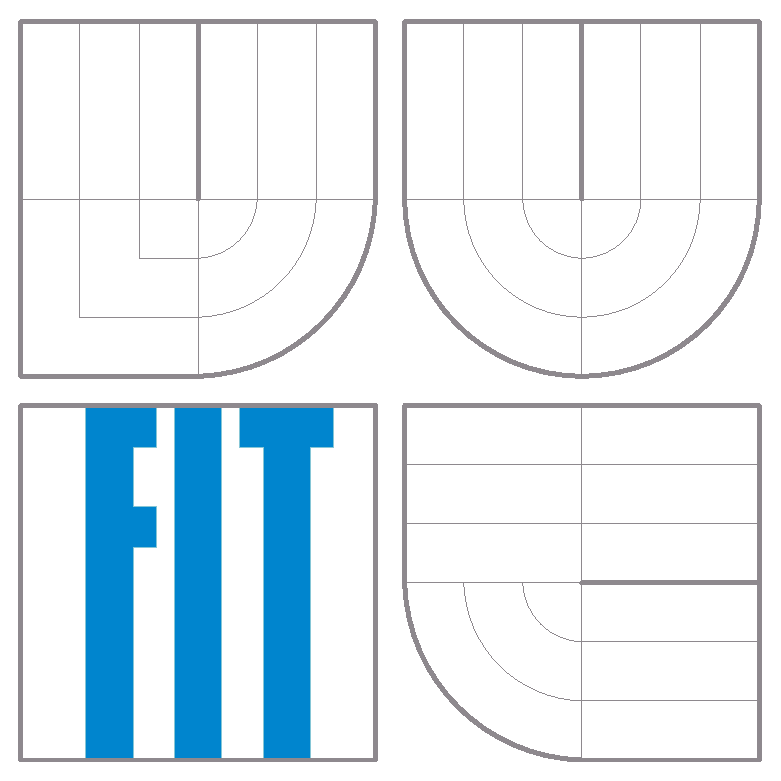
\includegraphics[height=5cm]{img/logo.eps}
\end{figure}

\vfill

\begin{center}
\begin{Large}
Dokumentácia projektu\\
\end{Large}

\bigskip

	\begin{Huge}
		\projname\\
	\end{Huge}

	\begin{large}
		Varianta a/1/II\\
		{\small Rozšírenia MINUS, BASE, REPEAT, FUNEXP, ELSEIF, BOOLOP \par}
	\end{large}
\end{center}

\vfill

\begin{center}
\begin{Large}
\today
\end{Large}
\end{center}

\vfill

\begin{flushleft}

	\begin{large}
		\begin{tabularx}{\linewidth}{Xlr}
		   & \textbf{Vedúci týmu 002:} & \textbf{Dávid Mikúš (xmikus15)} \\
		   & Členovia: & Peter Hostačný (xhosta03) \\
		   &           & Tomáš Kello (xkello00) \\
		   &           & Adam Lučanský (xlucan01) \\
		   &           & Michaela Lukášova (xlukas09)
		\end{tabularx}
	\end{large}
\end{flushleft}
\end{titlepage}


%%%%%%%%%%%%%%%%%%%%%%%%%%%%%%%%%%%%%%%%%%%%%%%%%%%%%%%%%%%%%%%%%%%%%%%%%%%%%%
% obsah
\pagestyle{plain}
\pagenumbering{roman}
\setcounter{page}{1}
\tableofcontents

\listoftodos[Notes]

%%%%%%%%%%%%%%%%%%%%%%%%%%%%%%%%%%%%%%%%%%%%%%%%%%%%%%%%%%%%%%%%%%%%%%%%%%%%%%
% textova zprava
\newpage
\pagestyle{plain}
\pagenumbering{arabic}
\setcounter{page}{1}

%%%%%%%%%%%%%%%%%%%%%%%%%%%%%%%%%%%%%%%%%%%%%%%%%%%%%%%%%%%%%%%%%%%%%%%%%%%%%%
\section{Úvod} \label{uvod}
%%%%%%%%%%%%%%%%%%%%%%%%%%%%%%%%%%%%%%%%%%%%%%%%%%%%%%%%%%%%%%%%%%%%%%%%%%%%%%

\todo[inline]{Vymyslieť text}

%%%%%%%%%%%%%%%%%%%%%%%%%%%%%%%%%%%%%%%%%%%%%%%%%%%%%%%%%%%%%%%%%%%%%%%%%%%%%%
\section{Riešenie projektu} \label{riesenie}
%%%%%%%%%%%%%%%%%%%%%%%%%%%%%%%%%%%%%%%%%%%%%%%%%%%%%%%%%%%%%%%%%%%%%%%%%%%%%%

\subsection{Interpret}

\subsection{Algoritmy}
	\todo[inline]{Sem dopíše Tomáš postupy postupy riešenia algoritmov etc.}

\subsection{Práca v tíme}
%%%%%%%%%%%%%%%%%%%%%%%%%%%%%%%%%%%%%%%%%%%%%%%%%%%%%%%%%%%%%%%%%%%%%%%%%%%%%%
% přílohy
\appendix

\section{Metriky kódu} \label{metriky}
\paragraph{Počet riadkov zdrojového textu:} 12689 riadkov
\paragraph{Veľkosť statických dát:} 6147B
\paragraph{Veľkosť spustiteľného programu:} 13294B
\todo[inline]{Aktualizovať metriky po dopísani projektu}

%
\section{LL Gramatika} \label{gramatika}

%
\section{Precedenčná tabuľka} \label{precedencna_tabulka}

\newcommand{\la}{\langle}
\newcommand{\ra}{\rangle}
\begin{table}[ht]
\begin{tabular}{c|ccccccccccccccccccccc}
                & U- & not & * & / & and & + & - & or & xor & $\lang$ & $\rang$ & $\lang$ = & $\rang$ = & = & $\lang$ $\rang$ & ( & ) & f & , & \$ & var \\ \hline
U-              & H  &  R  & R & R &  R  & R & R & R  &  R  &   R     &    R    & R  & R  & R & R  & S & R & S & R & R  & S   \\ %  U-
not             & R  &  H  & R & R &  R  & R & R & R  &  R  &   R     &    R    & R  & R  & R & R  & S & R & S & R & R  & S   \\ % not
*               & S  &  S  & R & R &  R  & R & R & R  &  R  &   R     &    R    & R  & R  & R & R  & S & R & S & R & R  & S   \\ %  *
/               & S  &  S  & R & R &  R  & R & R & R  &  R  &   R     &    R    & R  & R  & R & R  & S & R & S & R & R  & S   \\ %  /
and             & S  &  S  & R & R &  R  & R & R & R  &  R  &   R     &    R    & R  & R  & R & R  & S & R & S & R & R  & S   \\ % and
+               & S  &  S  & S & S &  S  & R & R & R  &  R  &   R     &    R    & R  & R  & R & R  & S & R & S & R & R  & S   \\ %  +
-               & S  &  S  & S & S &  S  & R & R & R  &  R  &   R     &    R    & R  & R  & R & R  & S & R & S & R & R  & S   \\ %  -
or              & S  &  S  & S & S &  S  & R & R & R  &  R  &   R     &    R    & R  & R  & R & R  & S & R & S & R & R  & S   \\ %  or
xor             & S  &  S  & S & S &  S  & R & R & R  &  R  &   R     &    R    & R  & R  & R & R  & S & R & S & R & R  & S   \\ % xor
$\lang$         & S  &  S  & S & S &  S  & S & S & S  &  S  &   R     &    R    & R  & R  & R & R  & S & R & S & R & R  & S   \\ %  <
$\rang$         & S  &  S  & S & S &  S  & S & S & S  &  S  &   R     &    R    & R  & R  & R & R  & S & R & S & R & R  & S   \\ %  >
$\lang$ =       & S  &  S  & S & S &  S  & S & S & S  &  S  &   R     &    R    & R  & R  & R & R  & S & R & S & R & R  & S   \\ %  <=
$\rang$ =       & S  &  S  & S & S &  S  & S & S & S  &  S  &   R     &    R    & R  & R  & R & R  & S & R & S & R & R  & S   \\ %  >=
=               & S  &  S  & S & S &  S  & S & S & S  &  S  &   R     &    R    & R  & R  & R & R  & S & R & S & R & R  & S   \\ %  =
$\lang$ $\rang$ & S  &  S  & S & S &  S  & S & S & S  &  S  &   R     &    R    & R  & R  & R & R  & S & R & S & R & R  & S   \\ %  <>
(               & S  &  S  & S & S &  S  & S & S & S  &  S  &   S     &    S    & S  & S  & S & S  & S & H & S & H & E  & S   \\ %  (
)               & R  &  R  & R & R &  R  & R & R & R  &  R  &   R     &    R    & R  & R  & R & R  & E & R & E & R & R  & E   \\ %  )
f               & E  &  E  & E & E &  E  & E & E & E  &  E  &   E     &    E    & E  & E  & E & E  & H & E & E & E & E  & E   \\ %  f
,               & S  &  S  & S & S &  S  & S & S & S  &  S  &   S     &    S    & S  & S  & S & S  & S & H & S & H & E  & S   \\ %  ,
\$              & S  &  S  & S & S &  S  & S & S & S  &  S  &   S     &    S    & S  & S  & S & S  & S & E & S & E & E  & S   \\ %  $
var             & R  &  R  & R & R &  R  & R & R & R  &  R  &   R     &    R    & R  & R  & R & R  & E & R & E & R & R  & E      % var
\end{tabular}
\end{table}






\end{document}
